\documentclass[a0paper,fleqn]{betterposter/betterposter}
\usepackage{hyperref}
\usepackage{hyperxmp}
\usepackage{pythonhighlight}
\usepackage[
    type={CC},
    modifier={by},
    version={3.0},
]{doclicense}
\lstset{
language = Python,
backgroundcolor={\color[gray]{.95}},
breaklines = true,
basicstyle=\fontsize{30}{32}\selectfont\ttfamily,
commentstyle = {\itshape \color[cmyk]{1,0.4,1,0}},
keywordstyle = {\bfseries \color[cmyk]{0,1,0,0}},
stringstyle = {\ttfamily \color[rgb]{1,0,0}},
}

\begin{document}
\betterposter{

	\maincolumn{

		3D plotting and mesh analysis through a streamlined interface for the Visualization Toolkit (VTK)
	}{

		\qrcode{img/qrcode}{img/smartphoneWhite}{
			\textbf{Take a picture} to
			\\visit the tutorial website
		}
		% Smartphone icon
		% Author: Freepik
		% Retrieved from: https://www.flaticon.com/free-icon/smartphone_65680

	}

}{

	
\includegraphics[width=\textwidth]{img/logo}\\

	\lstinputlisting[firstline=11, lastline=17]{hello-world.py}

	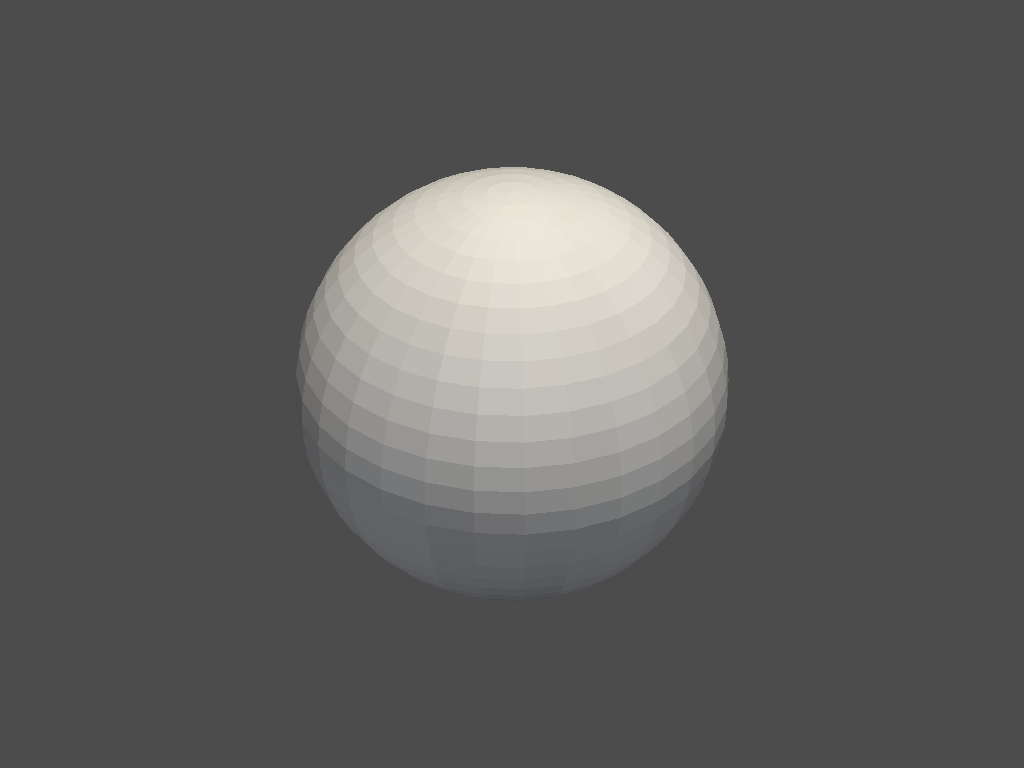
\includegraphics[width=\textwidth]{img/hello-world}

	\lstinputlisting[firstline=18, lastline=24]{hello-world.py}

	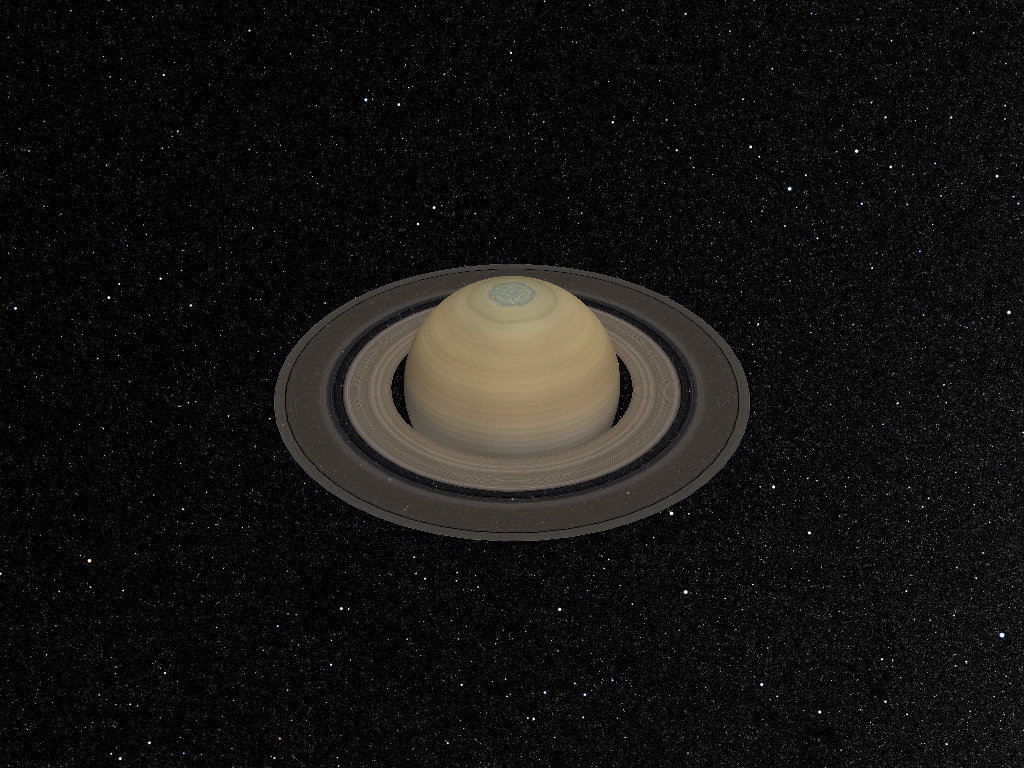
\includegraphics[width=\textwidth]{img/saturn}

	\lstinputlisting[firstline=26, lastline=32]{hello-world.py}

	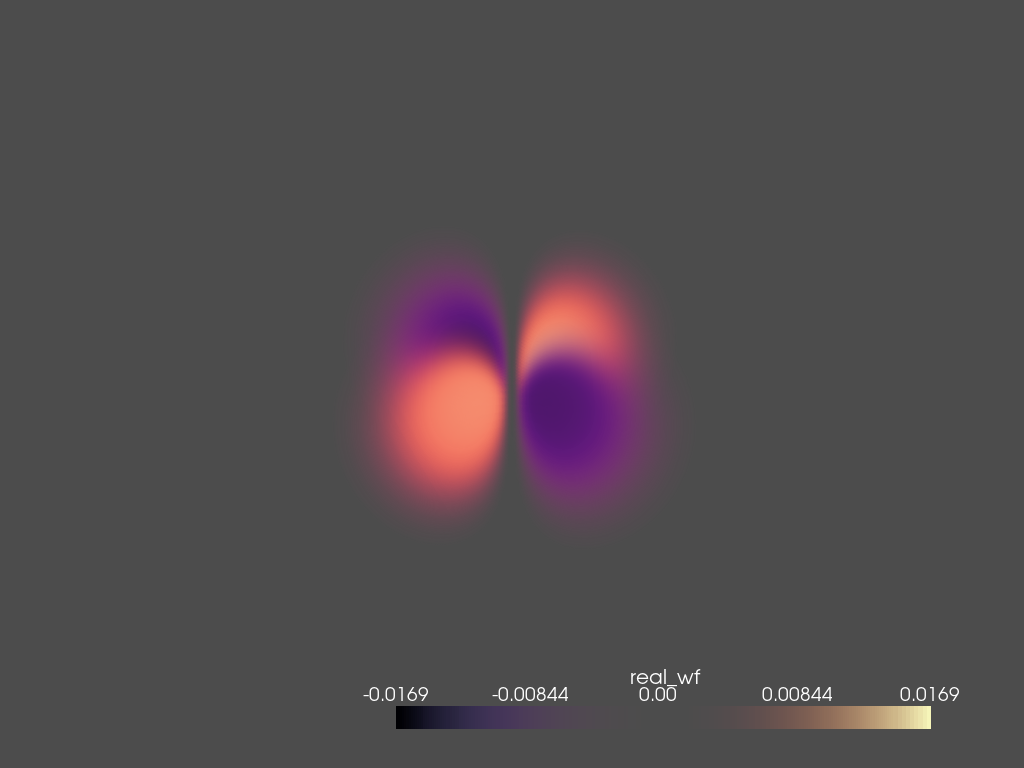
\includegraphics[width=\textwidth]{img/atom}

}{
	\section{PyVista Ecosystem}

	
\includegraphics[width=\textwidth]{img/logo-big}\\

	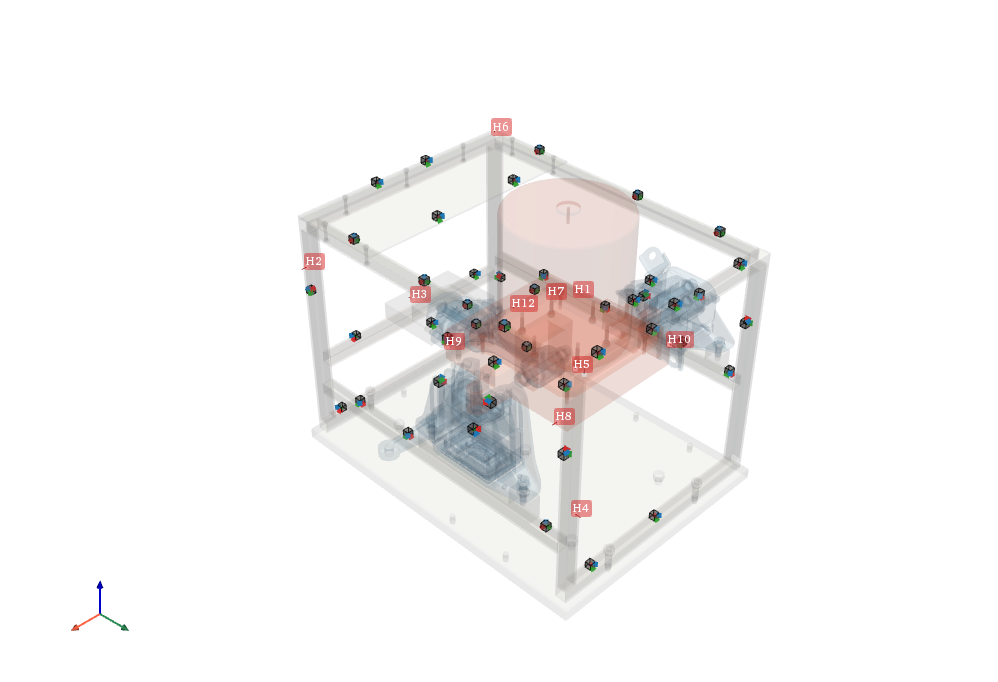
\includegraphics[width=\textwidth]{img/six_one}\\

	\qrcode{img/qrcode-pyfbs}{img/smartphoneBlack}{
		\textbf{Take a picture} to
		\\visit the pyFBS website
	}\\

	\vspace{60pt}

	
\includegraphics[width=\textwidth]{img/geovistalogo}\\

	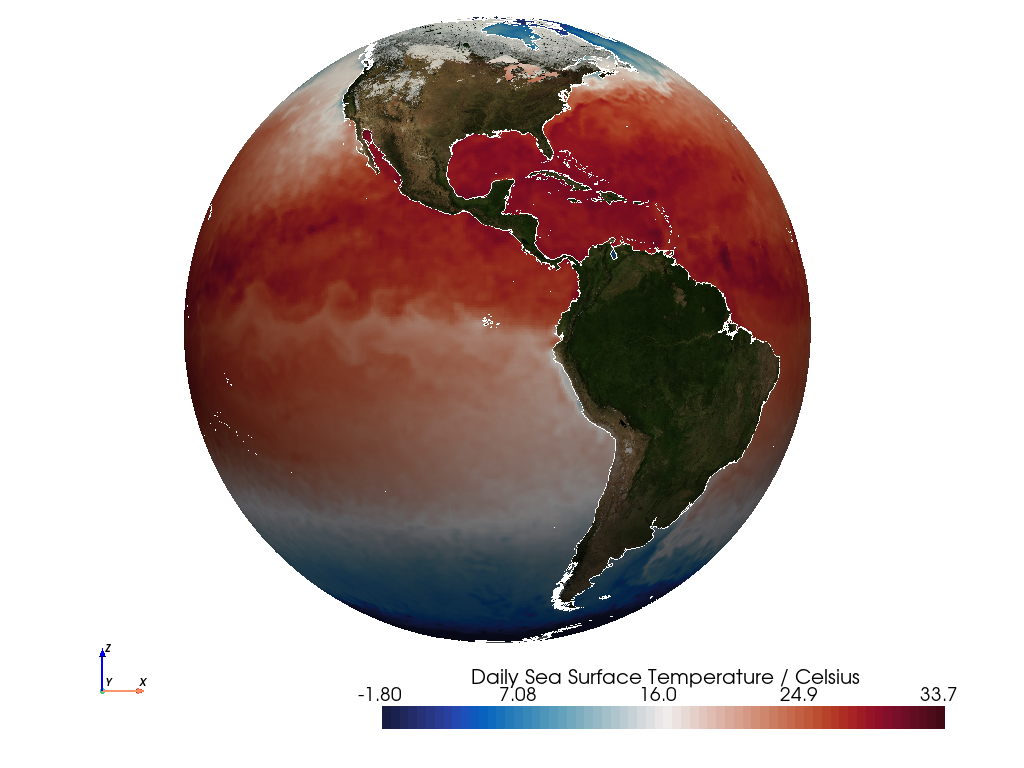
\includegraphics[width=\textwidth]{img/oisst-avhrr}\\

	\qrcode{img/qrcode-geovista}{img/smartphoneBlack}{
		\textbf{Take a picture} to
		\\visit the GeoVista website
	}\\

	\vspace{60pt}

	\doclicenseLongText\\

	\begin{center}
		\doclicenseImage\\
		\author{PyVista Project}
	\end{center}

}
\end{document}
